\subsection{Mechanistic circuit evidence (TRM minimal)}

Following Section~4 of \citet{nanda2023progress}, we reverse-engineer the grokked minimal TRM using $W_L$ Fourier maps, MLP neuron clustering, and attention routing (Figures~\ref{fig:wl}--\ref{fig:attn}).

At the best-FVE checkpoint (seed~0: step~5000, faithful FVE $\approx 0.96$), five key frequencies dominate excluded-loss sensitivity.
Per-neuron tables (Figure~\ref{fig:neuron_hist}) show concentration of MLP units on $\cos/\sin(\omega_k(a+b))$ features.
The all-frequency ablation grid (Figure~\ref{fig:all_freq}) confirms causal dependence on a sparse frequency subset.

\begin{figure}[h]
  \centering
  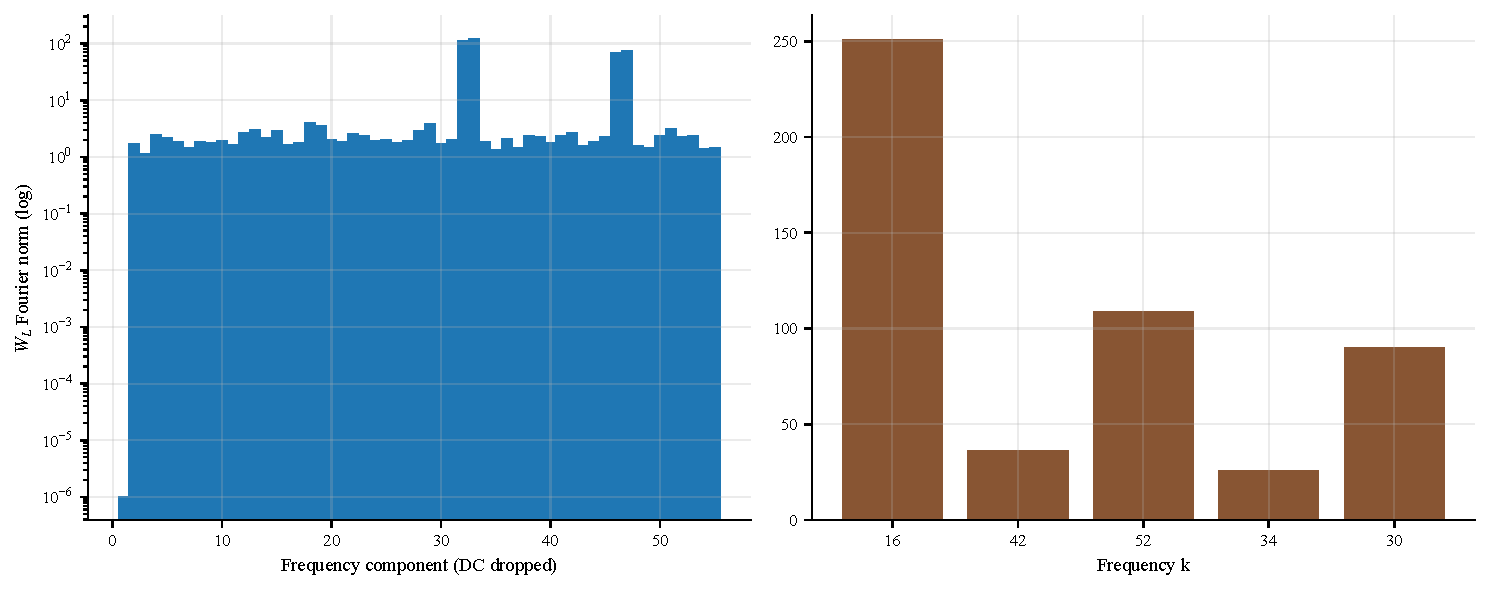
\includegraphics[width=0.95\linewidth]{figures/fig_wl_mlp_reverse_engineering.pdf}
  \caption{$W_L$ Fourier norms and neuron counts per key frequency (TRM minimal seed~0).}
  \label{fig:wl}
\end{figure}

\begin{figure}[h]
  \centering
  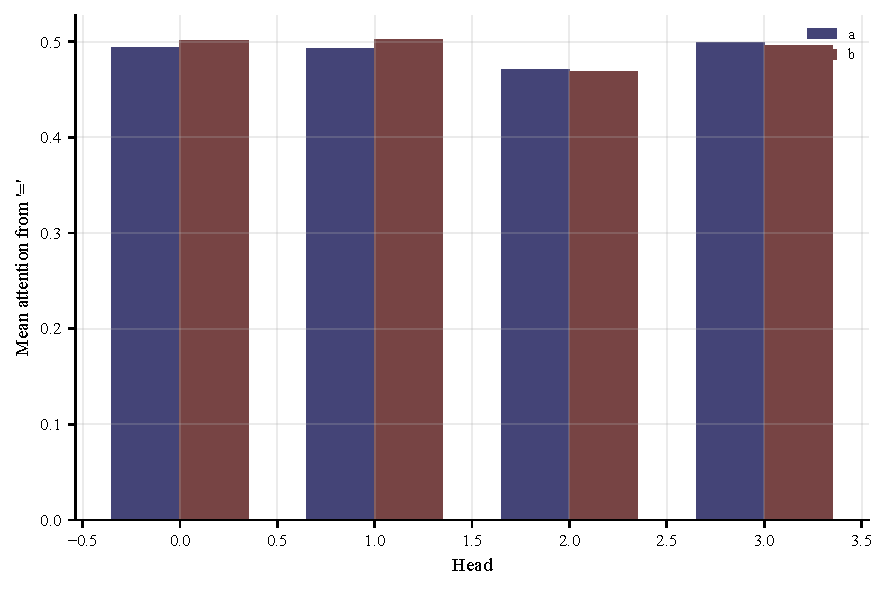
\includegraphics[width=0.7\linewidth]{figures/fig_attention_decomposition.pdf}
  \caption{Attention from ``$=$'' to operand tokens (layer~0).}
  \label{fig:attn}
\end{figure}

\begin{figure}[h]
  \centering
  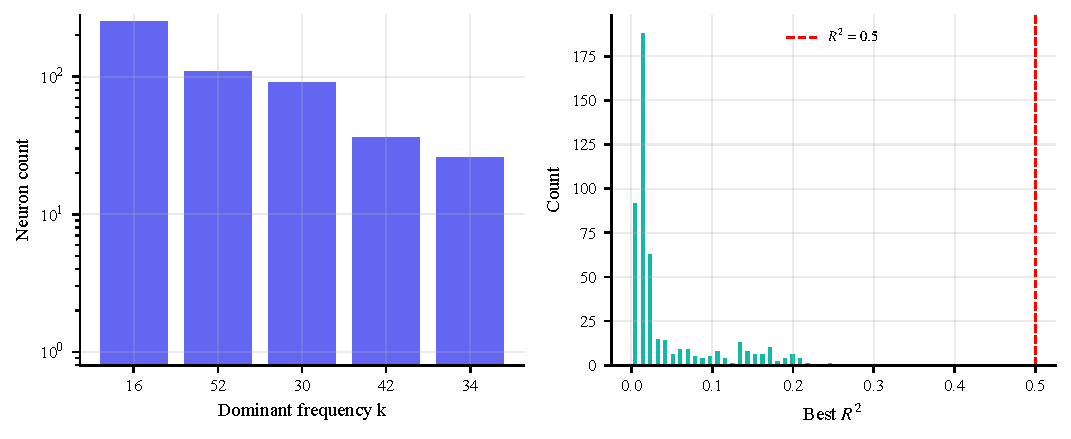
\includegraphics[width=0.95\linewidth]{figures/fig_neuron_frequency_tables.pdf}
  \caption{Per-neuron dominant frequency histogram and $R^2$ distribution.}
  \label{fig:neuron_hist}
\end{figure}

\paragraph{Seed variance diagnosis.}
Multi-seed training reveals that final-checkpoint FVE can collapse during the cleanup phase even when test accuracy remains at 100\% (Table~\ref{tab:seed_variance}, Appendix~\ref{app:seeds}).
We therefore report \textbf{three checkpoint types}: final, first grokking ($\geq 99\%$ acc, low loss), and best faithful FVE among high-accuracy steps (Table~\ref{tab:checkpoint_compare}).
The main Nanda-grade mechanistic claim rests on best-FVE / grokking checkpoints (mean best-FVE FVE $\HybridMinimalFVEBest$), not degraded finals ($\HybridMinimalFVE$).
